\documentclass[border=12pt]{standalone}
\usepackage[utf8]{inputenc}
\usepackage[utf8]{vietnam}
\usepackage{amsmath,amsfonts,amssymb}
\usepackage{tikz}
\usetikzlibrary{arrows, decorations.markings, calc, fadings, decorations.pathreplacing, patterns, decorations.pathmorphing, positioning}

\begin{document}
    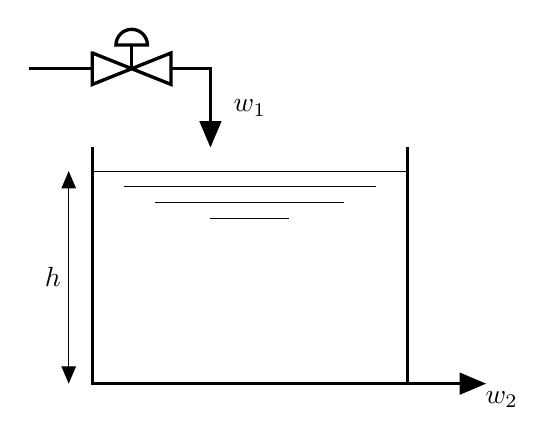
\begin{tikzpicture}[>=triangle 45]
        % Vẽ bình chứa
        \draw[line width=1.2pt] (0,3) -- (0,0) -- (4,0) -- (4,3);
        \draw (0,2.7) -- (4,2.7);
        \draw (0.4,2.5) -- (3.6, 2.5);
        \draw (0.8,2.3) -- (3.2, 2.3);
        \draw (1.5,2.1) -- (2.5, 2.1);
        \draw[line width=1.2pt] (-.8, 4) -- (0,4);
        \draw[line width=1.2pt] (0,4.2) -- (1,3.8) -- (1,4.2) -- (0,3.8) -- (0,4.22);
        \draw[line width=1.2pt] (0.5,4) -- (0.5, 4.3);
        \draw[line width=1.2pt] (0.7,4.3) arc (0:180:0.2) -- (0.72,4.3);
        \draw[line width=1.2pt] (1,4) -- (1.52,4);
        \draw[line width=1.2pt, ->] (1.5, 4) -- (1.5, 3);
        \draw (2, 3.5) node{$w_1$};

        \draw[<->] (-0.3,0) -- (-0.3,2.7);
        \draw (-0.5, 1.35) node {$h$};

        % Vẽ ngõ ra
        \draw[line width=1.2pt, ->] (4,0) -- (5,0);
        \draw (5.2,-.2) node{$w_2$};
    \end{tikzpicture}
\end{document}
